\documentclass[twoside,10pt]{report}
\usepackage{/Users/bradenhoagland/latex/styles/toggles}
\toggletrue{sectionbreaks}
\newcommand{\docTitle}{Stochastic Calculus}
\usepackage{/Users/bradenhoagland/latex/styles/common}
\importStyles{formal}{rainbow}{boxy}

%\renewcommand{\theenumi}{\alph{enumi}}

\begin{document}
\tableofcontents

%+-------------------+
%| +---------------+ |
%| |    Chapter    | |
%| +---------------+ |
%+-------------------+
% Basics

\chapter{Basics}

\warn{variation, quadratic variation}

\warn{filtration}

%--------------------------------------------------------------------------------
% Continuity
%--------------------------------------------------------------------------------
\section{Continuity}

\begin{defn}[]
A function $f:I\to \R$ is $\gamma$-\textbf{H\"older continuous} if there is a $C < \infty$ such that
\[
|f(t) - f(s)| \leq C \; |t-s|^{\gamma}
\] for all $s,t \in I$. Functions with $\gamma=1$ are \textbf{Lipschitz continuous}.
\end{defn}

\begin{thrm}[Kolmogorov Continuity Theorem]
	Let $\left\{ X_{t} \right\}$ be a stochastic process on $[0,1]$. If there are $\alpha,\beta,C>0$ such that
	\[
	\E{ |X_{t}-X_{s}|^{\alpha} } \leq C |t-s|^{1+\beta},
	\] then there is a version $\tilde{X}_{t}$ of $X_{t}$ with sample paths that are almost surely $\gamma$-H\"older continuous for $\gamma \in (0, \beta/\alpha)$.
\end{thrm}

\warn{version means $\P{ \tilde{X}_{t}=X_{t} }=1$ for all $t$.}


%+-------------------+
%| +---------------+ |
%| |    Chapter    | |
%| +---------------+ |
%+-------------------+
% Brownian Motion

\chapter{Brownian Motion}

\begin{defn}[]
A standard \textbf{Brownian motion} $B(t,\omega)$ is a continuous time $\R$-valued stochastic process over some $(\Omega,\mathcal{F},\mathbb{P})$ such that
\begin{enumerate}
	\item $B_{t}-B_{s}\sim \mathcal{N}(0, t-s)$;
	\item Disjoint increments are independent;
	\item The sample path $t \mapsto B_{t}(\omega)$ is continuous with probability 1.
\end{enumerate}
\end{defn}

At all times, a Brownian motion receives an infinitesimal Gaussian kick. The intuition here is that ``$dB$" is then a Gaussian random variable. Of course, $dB$ is meaningless right now since $B$ is nowhere differentiable with probability 1, but we will give it meaning later in terms of It\^o integrals, and the interpretation will be the same.

A useful fact for proving that disjoint intervals are independent: two Gaussians are independent $\iff$ they have 0 covariance.

\begin{figure}[H]
	\centering
	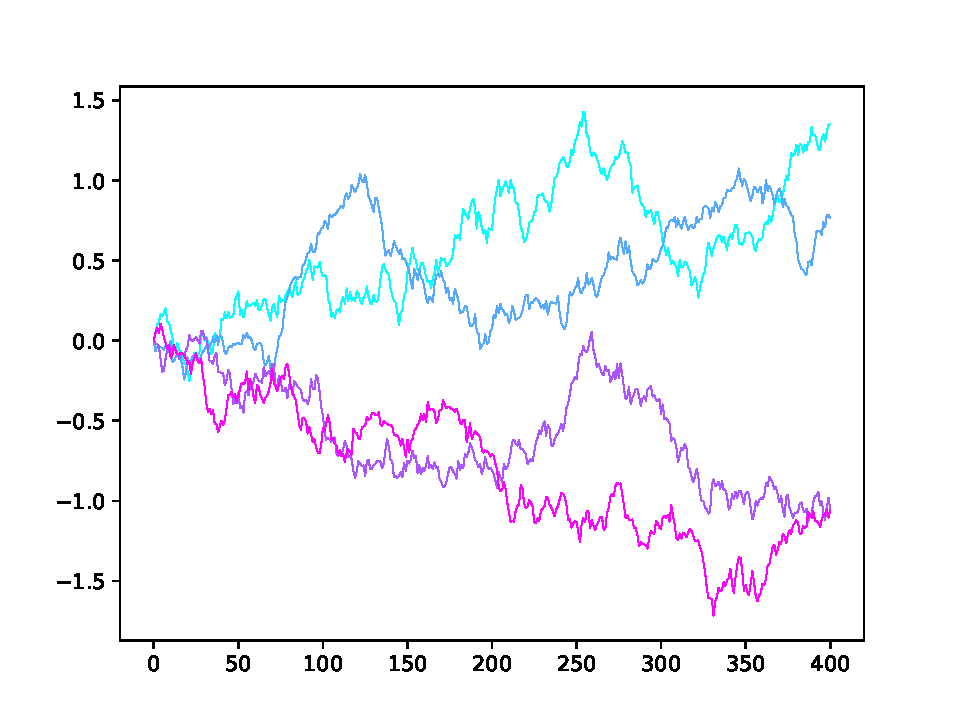
\includegraphics[scale=0.6]{fig/brownian.pdf}
	%\caption{}
\end{figure}

\begin{prop}
	If $B_{t}$ is a Brownian motion, then so are the following two processes:
	\begin{itemize}
		\item $X_{t} := \frac{1}{\sqrt{\alpha} } B_{\alpha t}$ for fixed $\alpha > 0$;
		\item $Y_{t} := B_{s+t} - B_{s}$ for fixed $s>0$;
		\item $Z_{t} := t B_{1/t}$.
	\end{itemize}
\end{prop}

\begin{prop}
If $B_{t}$ is a Brownian motion, then $\cov(B_{t},B_{s}) = \min(t,s)$.
\end{prop}

\warn{Construct a BM using Wiener measure and $B_{t}(\omega) = \omega_{t}$.}

\warn{Is the following the finite dimensional distribution stuff?}

Let $ A := \left\{ \omega \;|\; B_{t_k}(\omega) \in (a_{k},b_{k}) \text{ for } k=1,\dots,N \right\}$. If
\[
\phi(s,y) := \frac{\exp\left( -y^2/(2s) \right)}{\sqrt{2 \pi s^2} } ,
\] then the probability of $A$ is
\[
\P{ A } = \int_{a_1}^{b_1} \cdots \int_{a_n}^{b_n} \phi(t_1, x_1) \prod_{i=2}^{N} \phi(t_{i}-t_{i-1},x_{i}-x_{i-1}) \; dx_1\;\cdots\; dx_{n}.
\] The idea here is that $\phi(t_{i}-t_{i-1},x_{i}-x_{i-1})$ is the conditional density for $B_{t_k}$ given $B_{t_{k-1}}=x_{k-1}$.

\begin{prop}
	The sample paths of Brownian motion are almost surely $\gamma$-H\"older continuous for $\gamma \in (0,1/2)$.
\end{prop}

\begin{prop}
If $B$ is a Brownian motion on $[0,T]$, then with probability 1,
\begin{itemize}
	\item $V^{p}(B,[0,T]) < \infty$ for $p>2$;
	\item $V^{p}(B,[0,T]) = \infty$ for $p<2$.
\end{itemize}
The quadratic variation of $B$ is $[B,B](t) = t$.
\end{prop}

%+-------------------+
%| +---------------+ |
%| |    Chapter    | |
%| +---------------+ |
%+-------------------+
% Integration

\chapter{Integration}

%--------------------------------------------------------------------------------
% Integration of Simple Processes
%--------------------------------------------------------------------------------
\section{Integration of Simple Processes}

Suppose $B_{t}$ is a Brownian motion adapted to $\left\{ \mathcal{F}_{t} \right\}$. Then $\mathcal{L}_{A}^2([0,T] \times \Omega)$ is the space of all processes $X(t,\omega)$ adapted to $\left\{ \mathcal{F}_{t} \right\}$ such that
\[
\E{ \int_{0}^{T} X^2\;ds }< \infty.
\] This space is Banach space (complete normed vector space) with norm
\[
{\Vert{X}\Vert}_{\mathcal{L}_{A}^2} = \sqrt{\E{ \int_{0}^{T} X^2\;ds }} .
\] 
The subspace $\mathcal{L}_{A,0}^2 \subset \mathcal{L}_{A}^2$ of \emph{simple} adapted processes is dense in $\mathcal{L}_{A}^2$: for any $X \in \mathcal{L}_{A}^2$, there is a sequence $\left\{ X_{n} \right\} \subset \mathcal{L}_{A,0}^2$ converging to $X$ in the $\mathcal{L}^2$ sense, i.e.
\[
\lim_{n \to \infty} {\Vert{X_{n}-X}\Vert}_{\mathcal{L}_{A}^2} = \lim_{n \to \infty} \sqrt{\E{ \int_{0}^{T} (X_{n}-X)^2\;ds }} =0.
\] 
We'll define the It\^o integral for simple adapted processes, then extend it to general adapted processes in the next section.

\warn{finish}

\begin{prop}
Let $\sigma \in \mathcal{L}_{A}^2$, then the quadratic variation of $X(t) = \int_{0}^{t} \sigma\;dB$ is
\[
[X,X](t) = \int_{0}^{t} \sigma^{2}\;ds.
\] 
Note that if $\sigma$ depends on $\omega$, then $[X,X](t)$ is still a random variable.
\end{prop}

%--------------------------------------------------------------------------------
% Extending the It\^o Integral
%--------------------------------------------------------------------------------
\section{Extending the It\^o Integral}

For $X \in \mathcal{L}_{A}^2$, we know there's a sequence $ \left\{ X_{n} \right\}$ converging to $X$ in the $\mathcal{L}^2$ sense. Then by the It\^o isometry, the sequence $\left\{ I_{n} \right\}$ given by
\[
I_{n} := \int_{0}^{T} X_{n}\;dB
\] is a Cauchy sequence. Thus there is a random variable $I \in L^2$ such that $I_{n}\to I$ in the $L^2$ sense, i.e.
\[
\lim_{n \to \infty} {\Vert{I_{n}-I}\Vert}_{L^2} = \lim_{n \to \infty} \E{ |I_{n}-I|^2 } = 0.
\] 
\begin{defn}[]
For $X \in \mathcal{L}_{A}^2$,
\[
\int_{0}^{T} X\;dB
\] is the unique limit of the sequence given by $I_{n} := \int_{0}^{T} X_{n}\;dB$, where $X_{n} \to X$.
\end{defn}

This integral has all the same properties as the one for simple processes.
\warn{Further extension where martingale property becomes *local* martingal property.}

%--------------------------------------------------------------------------------
% It\^o Processes
%--------------------------------------------------------------------------------
\section{It\^o Processes}

\warn{do this.}

%--------------------------------------------------------------------------------
% It\^o's Formula
%--------------------------------------------------------------------------------
\section{It\^o's Formula}

\begin{thrm}[]
	Let $Z$ be an It\^o process satisfying
	\[
	dZ = \mu\;dt + \sigma\;dB.
	\] Let $f(t,x) \in C^2$, then
	\[
	df(t, Z_{t}) = \left[ \frac{\p f}{\p x} \right]dZ + \left[ \frac{\p f}{\p t} + \frac{1}{2} \frac{\p^2 f}{\p x^2} \sigma^{2} \right]dt,
	\] 
	where all partial derivatives are evaluated at $(t,Z_{t})$.
\end{thrm}


\end{document}
